\documentclass[]{tufte-handout}

% ams
\usepackage{amssymb,amsmath}

% utf8 encoding
\usepackage[utf8]{inputenc}

% graphix
\usepackage{graphicx}
\setkeys{Gin}{width=\linewidth,totalheight=\textheight,keepaspectratio}

% booktabs
\usepackage{booktabs}

% url
\usepackage{url}

% hyperref
\usepackage{hyperref}

% units.
\usepackage{units}

% pandoc syntax highlighting
\usepackage{color}
\usepackage{fancyvrb}
\newcommand{\VerbBar}{|}
\newcommand{\VERB}{\Verb[commandchars=\\\{\}]}
\DefineVerbatimEnvironment{Highlighting}{Verbatim}{commandchars=\\\{\}}
% Add ',fontsize=\small' for more characters per line
\newenvironment{Shaded}{}{}
\newcommand{\KeywordTok}[1]{\textcolor[rgb]{0.00,0.44,0.13}{\textbf{{#1}}}}
\newcommand{\DataTypeTok}[1]{\textcolor[rgb]{0.56,0.13,0.00}{{#1}}}
\newcommand{\DecValTok}[1]{\textcolor[rgb]{0.25,0.63,0.44}{{#1}}}
\newcommand{\BaseNTok}[1]{\textcolor[rgb]{0.25,0.63,0.44}{{#1}}}
\newcommand{\FloatTok}[1]{\textcolor[rgb]{0.25,0.63,0.44}{{#1}}}
\newcommand{\CharTok}[1]{\textcolor[rgb]{0.25,0.44,0.63}{{#1}}}
\newcommand{\StringTok}[1]{\textcolor[rgb]{0.25,0.44,0.63}{{#1}}}
\newcommand{\CommentTok}[1]{\textcolor[rgb]{0.38,0.63,0.69}{\textit{{#1}}}}
\newcommand{\OtherTok}[1]{\textcolor[rgb]{0.00,0.44,0.13}{{#1}}}
\newcommand{\AlertTok}[1]{\textcolor[rgb]{1.00,0.00,0.00}{\textbf{{#1}}}}
\newcommand{\FunctionTok}[1]{\textcolor[rgb]{0.02,0.16,0.49}{{#1}}}
\newcommand{\RegionMarkerTok}[1]{{#1}}
\newcommand{\ErrorTok}[1]{\textcolor[rgb]{1.00,0.00,0.00}{\textbf{{#1}}}}
\newcommand{\NormalTok}[1]{{#1}}

% longtable

% multiplecol
\usepackage{multicol}

% lipsum
\usepackage{lipsum}

% strikeout
\usepackage[normalem]{ulem}
 
% morefloats
\usepackage{morefloats}

% title / author / date
\title{WEB346}
\author{Benjamin Weigel}
\date{July 27th, 2015}


\begin{document}

\maketitle



\section{Question}\label{question}

Do Mg\textsuperscript{2+}, pH, chemical motif (e.g.~catecholic,
phenolic, 3'-OMe, 4'-OMe) and the choice of enzyme (WT or 4'-variant)
influence the observed conversion of flavonoids and phenylpropanoids by
the O-methyltransferase PFOMT?

\section{Introduction}\label{introduction}

17 different flavonoid and phenyl propanoid substrates were tested for
methylation. These substrates can loosely be categorized into four
groups by the chemical motif that is to be methylated (e.g.~catecholic,
phenolic, 3'-OMe, 4'-OMe). Three other factors are studied that might
also influence the conversion. The addition of Mg\textsuperscript{2+},
high (8.6) or low (7.5) pH and the enzyme variant (WT or 3'-variant)
that is used are also varied.

\newthought{A total of 96 experiments} were conducted to cover each
group at least with three independent observations.

\begin{marginfigure}
$$\mathrm{Mg} \times \mathrm{pH} \times \mathrm{variant} \times \mathrm{motif} $$
$$2 \times 2 \times 2 \times 4 = 32$$
\caption{number of groups studied}
\end{marginfigure}

\section{Results}\label{results}

\subsection{Data}\label{data}

\begin{table}[ht]
\centering
\begin{tabular}{rlrllll}
  \toprule
 & substrate & value & pH & Mg & variant & motif \\ 
  \midrule
1 & 1 & 0.00 & low & FALSE & WT & A \\ 
  2 & 1 & 0.00 & high & FALSE & Y51RN202W & A \\ 
  3 & 1 & 0.07 & high & TRUE & WT & A \\ 
  4 & 1 & 0.00 & low & TRUE & Y51RN202W & A \\ 
  5 & 1 & 0.04 & high & FALSE & WT & A \\ 
  6 & 1 & 0.00 & low & FALSE & Y51RN202W & A \\ 
   \bottomrule
\end{tabular}
\caption{First rows of dataframe} 
\end{table}

\begin{margintable}
\centering
\begin{tabular}{rll}
  \toprule
 & labels & motif \\ 
  \midrule
1 & A & phenolic \\ 
  2 & B & catecholic \\ 
  3 & C & 4-O-Me \\ 
  4 & D & 3-O-Me \\ 
   \bottomrule
\end{tabular}
\caption{Labels in the data.frame and their corresponding motif.} 
\end{margintable}

\subsection{Significance no enzyme
vs.~enzyme}\label{significance-no-enzyme-vs.enzyme}

Do the amounts of produced product vary significantly between treatments
were no enzyme was added and trreatm,ents with enzyme? Only ran blanks
at high pH with no magnesium added. Subset data to only include high pH,
no Mg, no catechols. The catechols were removed to avoid the bias
associated with an autocorrelation between product and catecholic
moiety.

\newthought{From the ANOVA table it is clear}, that conversion is not
due to chance. The p-value for the variant factor is almost 0. This
means, that we should be able to use the data for analyis.

\begin{Shaded}
\begin{Highlighting}[]
\KeywordTok{lm}\NormalTok{(value ~}\StringTok{ }\NormalTok{variant *}\StringTok{ }\NormalTok{motif, }\DataTypeTok{data =} \NormalTok{data.blank %>%}\StringTok{ }
\StringTok{    }\KeywordTok{filter}\NormalTok{(pH ==}\StringTok{ "high"}\NormalTok{, Mg ==}\StringTok{ }\NormalTok{F, motif !=}\StringTok{ "B"}\NormalTok{)) %>%}\StringTok{ }
\StringTok{    }\KeywordTok{aov}\NormalTok{() %>%}\StringTok{ }\KeywordTok{summary}\NormalTok{() %>%}\StringTok{ }\KeywordTok{xtable}\NormalTok{(., }\DataTypeTok{caption =} \StringTok{"ANOVA table for comparison of blanks and samples. There is a stitistical significance between treatments, where o enzyme was added and treatments that contained enzymne (the wt)."}\NormalTok{)}
\end{Highlighting}
\end{Shaded}

\begin{table}[ht]
\centering
\begin{tabular}{lrrrrr}
  \toprule
 & Df & Sum Sq & Mean Sq & F value & Pr($>$F) \\ 
  \midrule
variant       & 2 & 0.01 & 0.01 & 66.03 & 0.0000 \\ 
  motif         & 2 & 0.00 & 0.00 & 7.72 & 0.0038 \\ 
  variant:motif & 4 & 0.00 & 0.00 & 7.72 & 0.0008 \\ 
  Residuals     & 18 & 0.00 & 0.00 &  &  \\ 
   \bottomrule
\end{tabular}
\caption{ANOVA table for comparison of blanks and samples. There is a stitistical significance between treatments, where o enzyme was added and treatments that contained enzymne (the wt).} 
\end{table}\begin{figure}
 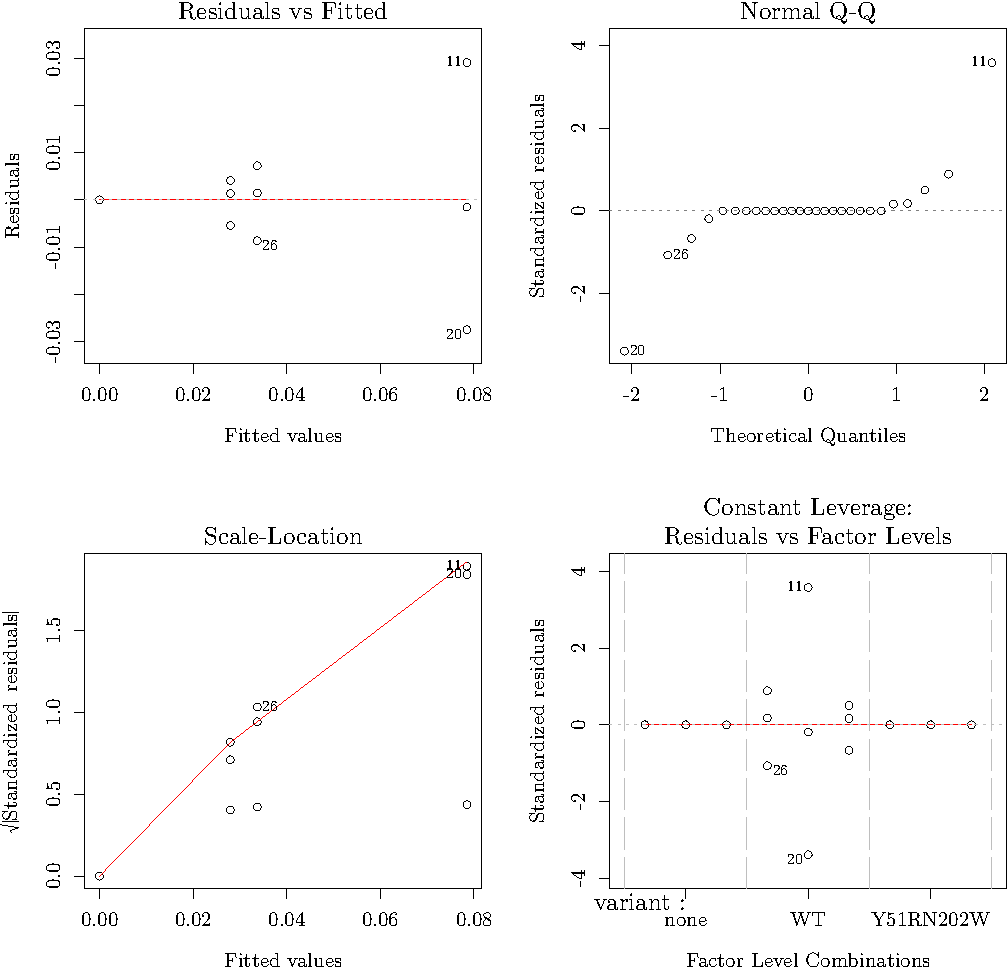
\includegraphics{tufte_files/figure-latex/unnamed-chunk-4-1.pdf}
\caption{Diagnostic plots of the ANOVA}
\end{figure}

\begin{marginfigure}
 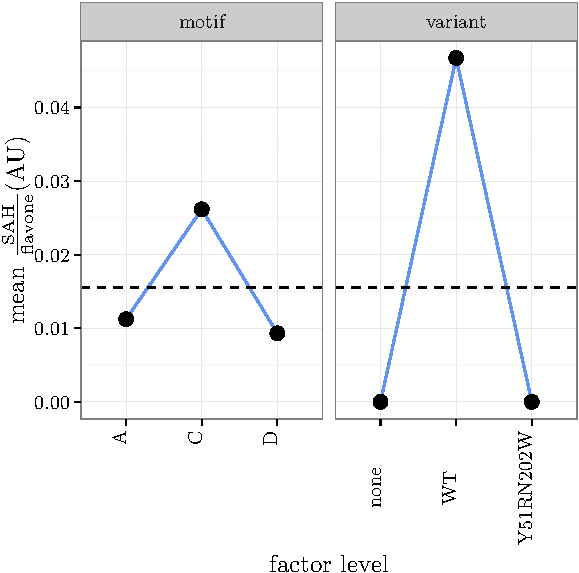
\includegraphics{tufte_files/figure-latex/unnamed-chunk-5-1.pdf}
\caption{Main effects plot for factors that influence product amount.}
\end{marginfigure}

\subsection{Main effects plots}\label{main-effects-plots}

The main effects plots (\ref{fig:mep}) give an overview of what happens.
The motif clearly has the biggest influence on conversion. This makes
sense, since PFOMT acts on catecholic moities.

\begin{figure}
 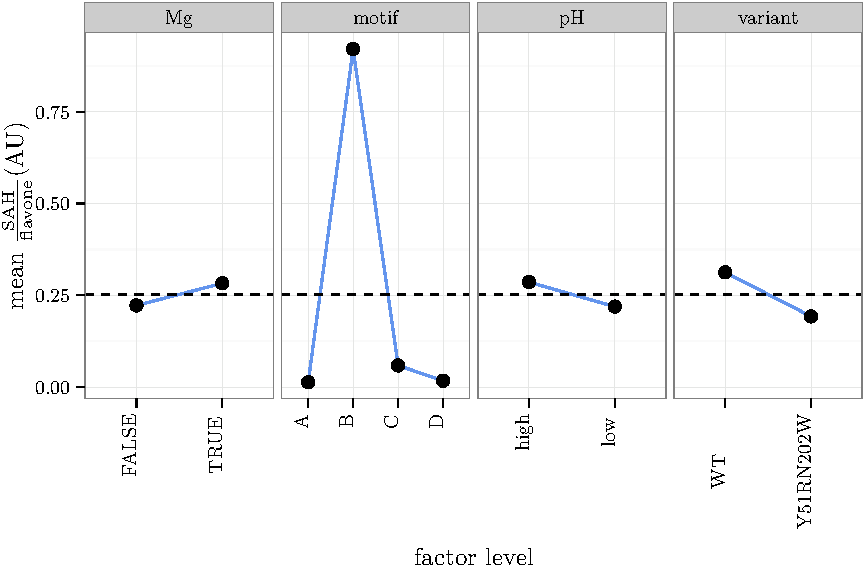
\includegraphics{tufte_files/figure-latex/MEP-1.pdf}
\caption{Main effetcs plots for the factor variables. Clearly the motif seems to have the biggest impact. Catecholic moieties are converted most effectively.}
\end{figure}\begin{figure}
 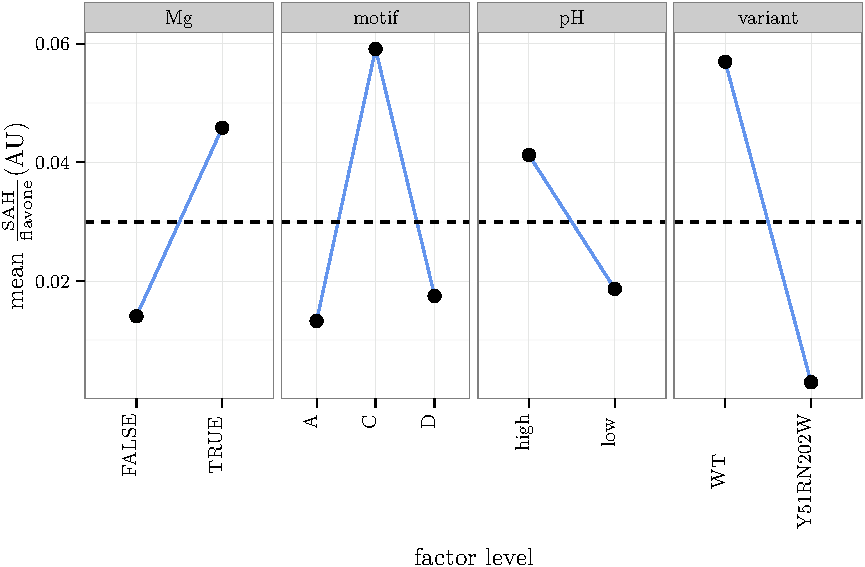
\includegraphics{tufte_files/figure-latex/MEP-2.pdf}
\caption{Main effects plot, when catecholic moieties factor is omitted. Phenolics are converted worst. The wildtype has the best activity.}
\end{figure}

\begin{marginfigure}
 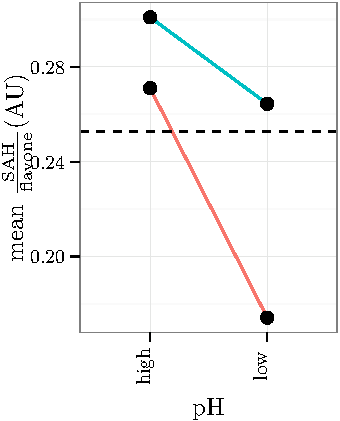
\includegraphics{tufte_files/figure-latex/IAP-1.pdf}
\caption{Interaction plot for Mg and pH. The lines suggest an interaction between pH and Mg, but this is not enough evidence to say wether that interaction is significant. red -- no magnesium, blue -- magnesium added.}
\end{marginfigure}

\newthought{The interaction plot}(\ref{fig:IAP}) of Mg and pH displays
an interaction. When magnesium is added the activity tends to be higher.
This effect is more pronounced at low pH values. It is not possible to
say wether this effect is significant without the according satistical
test. Indeed the ANOVA results suggest, that there is no significance.
In fact there doesn't even seem to be a statistical significance from Mg
addition or pH alone.

\subsection{Anova}\label{anova}

Two-way ANOVA test for simple models and more complex models were
prepared. The p-values for the complex model are very low all over.
However it is very likely that this is an overinterpretation of the
data. The data/experiment might be too complex to derive anything of
value from the information. The use of more complex modelling techniques
mnight shed some light. However, when the substrates with catecholic
moieties are excluded from the results, there is statistical
significance at leas for Mg and pH.

\begin{Shaded}
\begin{Highlighting}[]
\NormalTok{data.lm <-}\StringTok{ }\KeywordTok{lm}\NormalTok{(value ~}\StringTok{ }\NormalTok{pH *}\StringTok{ }\NormalTok{Mg, }\DataTypeTok{data =} \NormalTok{WEB346.results)}
\KeywordTok{summary}\NormalTok{(}\KeywordTok{aov}\NormalTok{(data.lm)) %>%}\StringTok{ }\KeywordTok{xtable}\NormalTok{(., }\DataTypeTok{caption =} \StringTok{"ANOVA table."}\NormalTok{)}
\end{Highlighting}
\end{Shaded}

\begin{table}[ht]
\centering
\begin{tabular}{lrrrrr}
  \toprule
 & Df & Sum Sq & Mean Sq & F value & Pr($>$F) \\ 
  \midrule
pH          & 1 & 0.11 & 0.11 & 0.61 & 0.4370 \\ 
  Mg          & 1 & 0.09 & 0.09 & 0.49 & 0.4837 \\ 
  pH:Mg       & 1 & 0.02 & 0.02 & 0.12 & 0.7247 \\ 
  Residuals   & 92 & 16.13 & 0.18 &  &  \\ 
   \bottomrule
\end{tabular}
\caption{ANOVA table.} 
\end{table}

\begin{Shaded}
\begin{Highlighting}[]
\NormalTok{data.lm <-}\StringTok{ }\KeywordTok{lm}\NormalTok{(value ~}\StringTok{ }\NormalTok{pH *}\StringTok{ }\NormalTok{Mg *}\StringTok{ }\NormalTok{motif *}\StringTok{ }\NormalTok{variant, }
    \DataTypeTok{data =} \NormalTok{WEB346.results)}
\KeywordTok{summary}\NormalTok{(}\KeywordTok{aov}\NormalTok{(data.lm)) %>%}\StringTok{ }\KeywordTok{xtable}\NormalTok{(., }\DataTypeTok{caption =} \StringTok{"ANOVA table of the most complex model. Significance is everywhere ... :O"}\NormalTok{)}
\end{Highlighting}
\end{Shaded}

\begin{table}[ht]
\centering
\begin{tabular}{lrrrrr}
  \toprule
 & Df & Sum Sq & Mean Sq & F value & Pr($>$F) \\ 
  \midrule
pH                  & 1 & 0.11 & 0.11 & 24.75 & 0.0000 \\ 
  Mg                  & 1 & 0.09 & 0.09 & 20.08 & 0.0000 \\ 
  motif               & 3 & 14.31 & 4.77 & 1105.42 & 0.0000 \\ 
  variant             & 1 & 0.35 & 0.35 & 80.19 & 0.0000 \\ 
  pH:Mg               & 1 & 0.02 & 0.02 & 5.07 & 0.0278 \\ 
  pH:motif            & 3 & 0.14 & 0.05 & 10.88 & 0.0000 \\ 
  Mg:motif            & 3 & 0.07 & 0.02 & 5.24 & 0.0027 \\ 
  pH:variant          & 1 & 0.03 & 0.03 & 7.14 & 0.0096 \\ 
  Mg:variant          & 1 & 0.02 & 0.02 & 3.52 & 0.0652 \\ 
  motif:variant       & 3 & 0.35 & 0.12 & 26.74 & 0.0000 \\ 
  pH:Mg:motif         & 3 & 0.08 & 0.03 & 6.49 & 0.0007 \\ 
  pH:Mg:variant       & 1 & 0.02 & 0.02 & 4.85 & 0.0313 \\ 
  pH:motif:variant    & 3 & 0.23 & 0.08 & 17.67 & 0.0000 \\ 
  Mg:motif:variant    & 3 & 0.20 & 0.07 & 15.29 & 0.0000 \\ 
  pH:Mg:motif:variant & 3 & 0.06 & 0.02 & 4.25 & 0.0084 \\ 
  Residuals           & 64 & 0.28 & 0.00 &  &  \\ 
   \bottomrule
\end{tabular}
\caption{ANOVA table of the most complex model. Significance is everywhere ... :O} 
\end{table}

\begin{Shaded}
\begin{Highlighting}[]
\NormalTok{data.lm <-}\StringTok{ }\KeywordTok{lm}\NormalTok{(value ~}\StringTok{ }\NormalTok{pH *}\StringTok{ }\NormalTok{Mg +}\StringTok{ }\NormalTok{variant, }\DataTypeTok{data =} \NormalTok{WEB346.results %>%}\StringTok{ }
\StringTok{    }\KeywordTok{filter}\NormalTok{(motif !=}\StringTok{ "B"}\NormalTok{))}
\KeywordTok{summary}\NormalTok{(}\KeywordTok{aov}\NormalTok{(data.lm)) %>%}\StringTok{ }\KeywordTok{xtable}\NormalTok{(., }\DataTypeTok{caption =} \StringTok{"ANOVA table when catecholics are excluded. At least the data suggest significance for pH and Mg."}\NormalTok{)}
\end{Highlighting}
\end{Shaded}

\begin{table}[ht]
\centering
\begin{tabular}{lrrrrr}
  \toprule
 & Df & Sum Sq & Mean Sq & F value & Pr($>$F) \\ 
  \midrule
pH          & 1 & 0.01 & 0.01 & 4.55 & 0.0366 \\ 
  Mg          & 1 & 0.02 & 0.02 & 9.01 & 0.0038 \\ 
  variant     & 1 & 0.05 & 0.05 & 26.07 & 0.0000 \\ 
  pH:Mg       & 1 & 0.00 & 0.00 & 0.14 & 0.7082 \\ 
  Residuals   & 67 & 0.13 & 0.00 &  &  \\ 
   \bottomrule
\end{tabular}
\caption{ANOVA table when catecholics are excluded. At least the data suggest significance for pH and Mg.} 
\end{table}

\subsection{Regression Tree}\label{regression-tree}

A regression tree can be built from the data. At first glance it shows,
that the motif is especially important for conversion. This is trivial,
since PFOMT is a 4'-OMT that acts on catecholic motifs. The substrates
with catecholic motifs are thus converted more efficiently.

\newthought{It seems as if the variant} is influenced by pH and metal
addition more clearly thatn the wt-enzyme, since the tree splits up
more.

\begin{figure}
 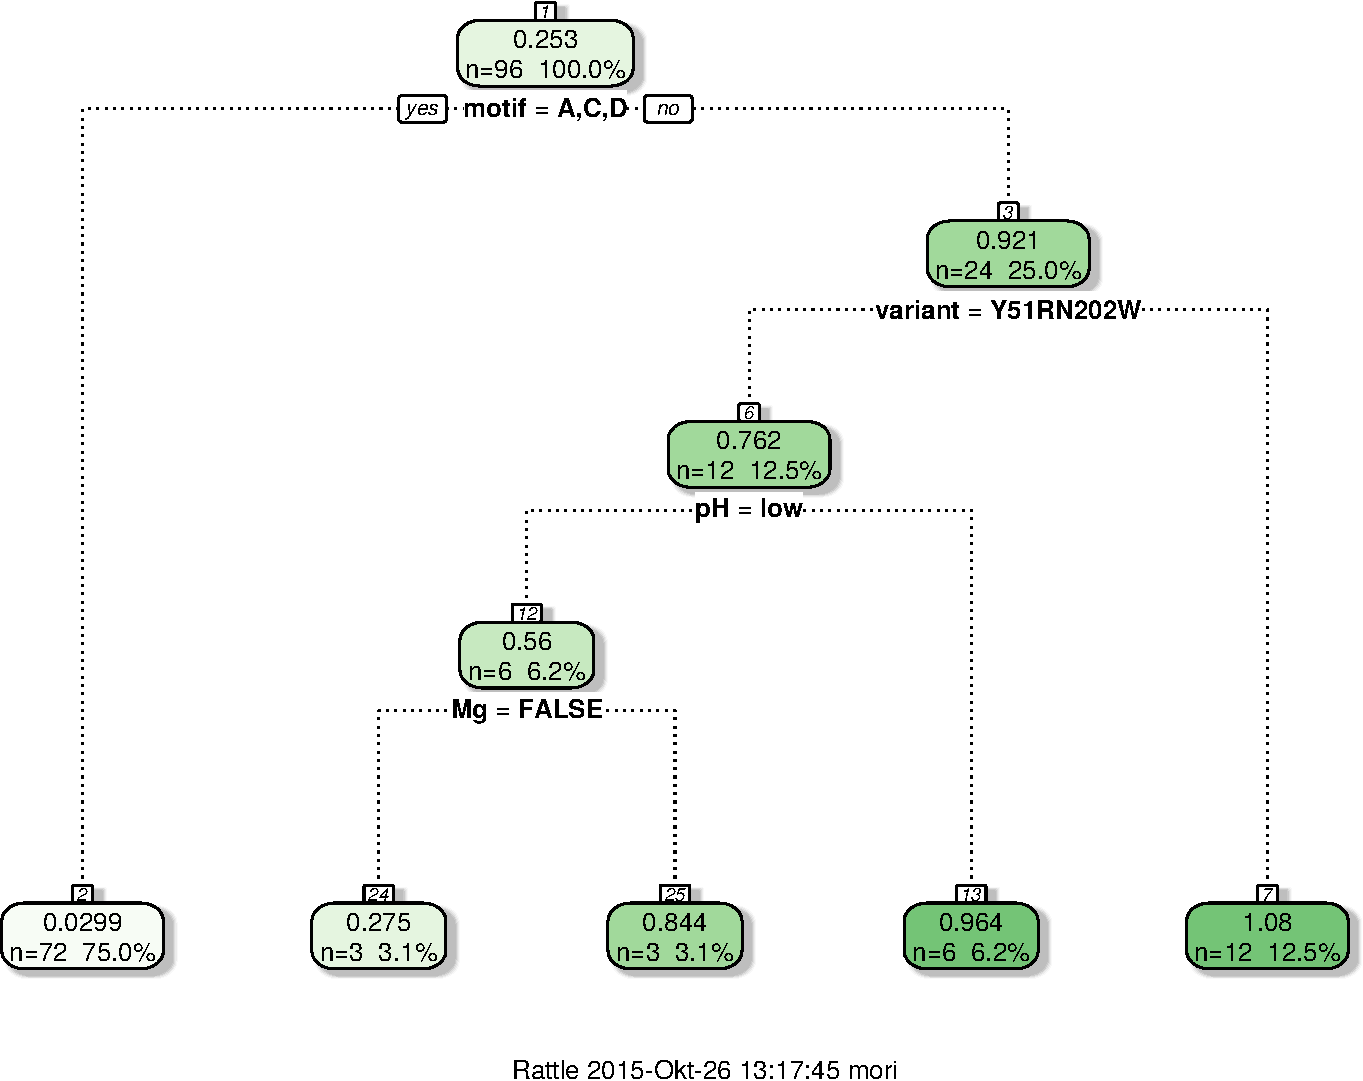
\includegraphics{tufte_files/figure-latex/unnamed-chunk-7-1.pdf}
\caption{RegressionTree of the data built with the `rpart`-package. The motif effects the conversion most. It seems that only the variant is influenced by pH and Mg.}
\end{figure}

\subsection{Linear Models}\label{linear-models}

At first it was checked, if pH and Mg have an influence on the
conversion. It does not seem that Mg or pH have any influence on the
conversion, as the p-values are much too high. This could be the result
of the fact that the conversion reactions were incubated for 16 hours.
Possible intricacies in the conversion (due to different reaction
velocities) can not be distinguished from one another if the reaction
time is so long that all substrate is used up.

\begin{table}[ht]
\centering
\begin{tabular}{rrrrr}
  \toprule
 & Estimate & Std. Error & t value & Pr($>$$|$t$|$) \\ 
  \midrule
(Intercept) & 0.2711 & 0.0855 & 3.17 & 0.0021 \\ 
  pHlow & -0.0969 & 0.1209 & -0.80 & 0.4247 \\ 
  MgTRUE & 0.0299 & 0.1209 & 0.25 & 0.8051 \\ 
  pHlow:MgTRUE & 0.0604 & 0.1709 & 0.35 & 0.7247 \\ 
   \bottomrule
\end{tabular}
\caption{A linear model with pH and Mg as factors is not a lot better than random guesses. p-values are very high. Thus this alone does not explain the variance.} 
\end{table}

\newthought{However, when the catecholics are omitted} as a factor level
it becomes clear that Mg and pH DO in fact influence the conversion.
After backwards selection only the factors pH, Mg, variant and te
interactions between variant and Mg and pH are retained.

\begin{Shaded}
\begin{Highlighting}[]
\NormalTok{data.lm <-}\StringTok{ }\KeywordTok{lm}\NormalTok{(value ~}\StringTok{ }\NormalTok{pH *}\StringTok{ }\NormalTok{Mg *}\StringTok{ }\NormalTok{variant, }\DataTypeTok{data =} \NormalTok{WEB346.results %>%}\StringTok{ }
\StringTok{    }\KeywordTok{filter}\NormalTok{(motif !=}\StringTok{ "B"}\NormalTok{))}
\NormalTok{data.lm <-}\StringTok{ }\NormalTok{MASS::}\KeywordTok{stepAIC}\NormalTok{(data.lm, }\DataTypeTok{direction =} \StringTok{"backward"}\NormalTok{)}
\end{Highlighting}
\end{Shaded}

\begin{verbatim}
## Start:  AIC=-447.48
## value ~ pH * Mg * variant
## 
##                 Df  Sum of Sq     RSS
## - pH:Mg:variant  1 6.5387e-05 0.11532
## <none>                        0.11526
##                     AIC
## - pH:Mg:variant -449.44
## <none>          -447.48
## 
## Step:  AIC=-449.44
## value ~ pH + Mg + variant + pH:Mg + pH:variant + Mg:variant
## 
##              Df Sum of Sq     RSS     AIC
## - pH:Mg       1 0.0002845 0.11561 -451.26
## <none>                    0.11532 -449.44
## - pH:variant  1 0.0075587 0.12288 -446.87
## - Mg:variant  1 0.0120562 0.12738 -444.28
## 
## Step:  AIC=-451.26
## value ~ pH + Mg + variant + pH:variant + Mg:variant
## 
##              Df Sum of Sq     RSS     AIC
## <none>                    0.11561 -451.26
## - pH:variant  1 0.0075587 0.12316 -448.70
## - Mg:variant  1 0.0120562 0.12766 -446.12
\end{verbatim}

\begin{table}[ht]
\centering
\begin{tabular}{lrrrrr}
  \toprule
 & Df & Sum Sq & Mean Sq & F value & Pr($>$F) \\ 
  \midrule
pH          & 1 & 0.01 & 0.01 & 5.23 & 0.0254 \\ 
  Mg          & 1 & 0.02 & 0.02 & 10.36 & 0.0020 \\ 
  variant     & 1 & 0.05 & 0.05 & 29.98 & 0.0000 \\ 
  pH:variant  & 1 & 0.01 & 0.01 & 4.32 & 0.0417 \\ 
  Mg:variant  & 1 & 0.01 & 0.01 & 6.88 & 0.0108 \\ 
  Residuals   & 66 & 0.12 & 0.00 &  &  \\ 
   \bottomrule
\end{tabular}
\caption{When catecholics are omitted there is significance in the following terms: pH, Mg, variant, pH:variant, Mg:variant} 
\end{table}

\marginnote{This is a margin note.  Notice that there isn't a number preceding the note.}

\begin{figure}
 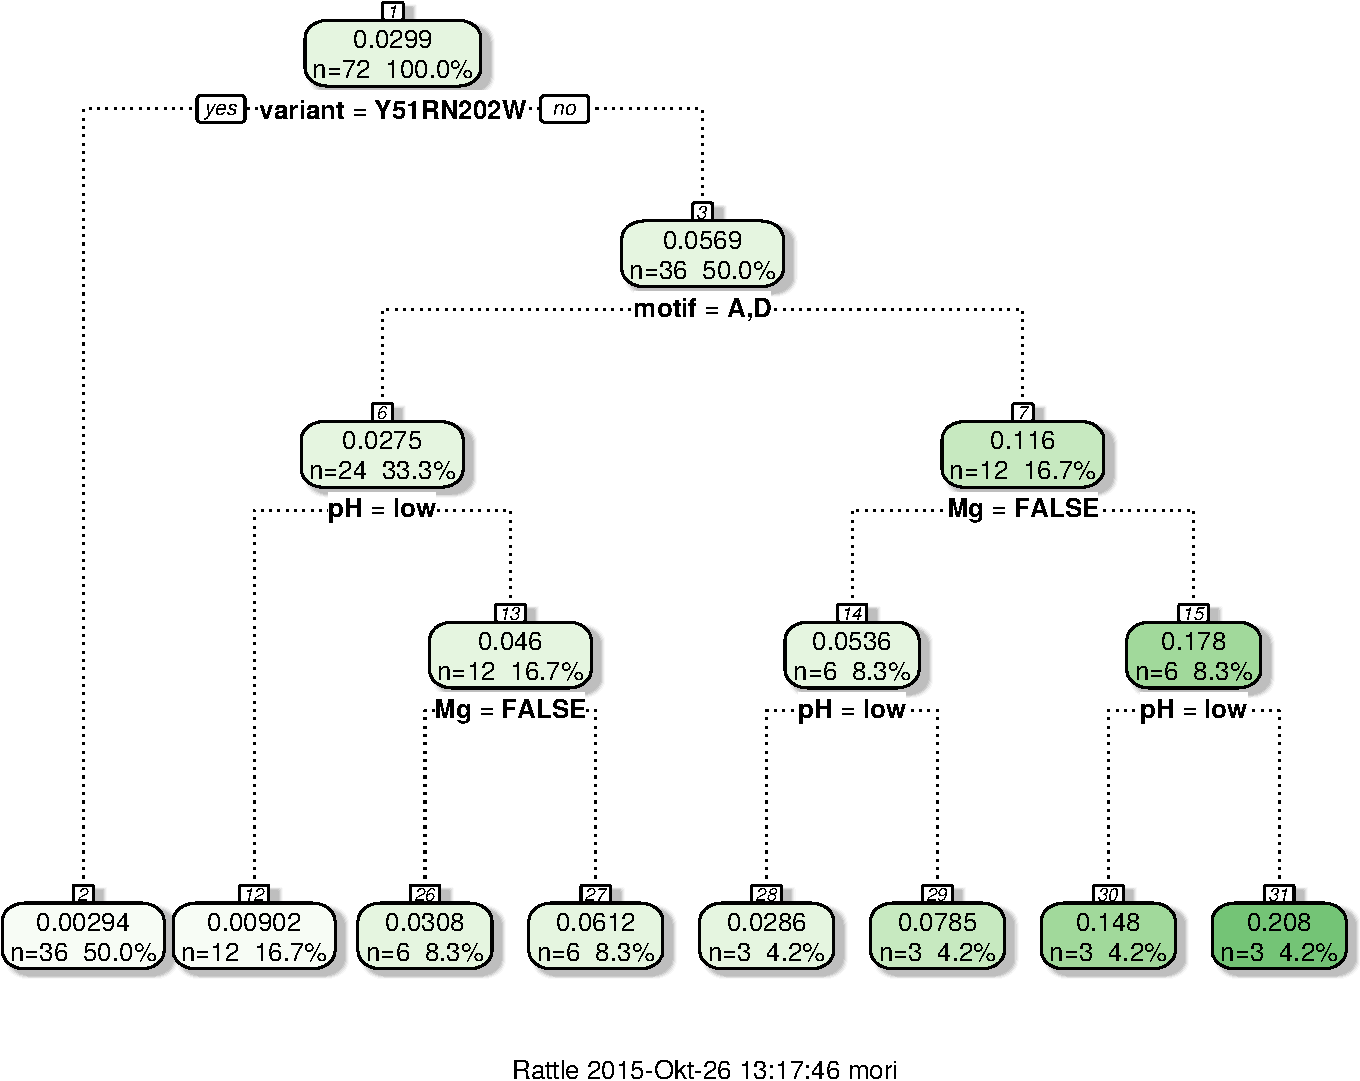
\includegraphics{tufte_files/figure-latex/regression_tree-1.pdf}
\caption{RegressionTree of the data of only substrates with phenolic, 3'-OMe and 4'-OMe moieties. Catecholic substrates are omitted.}
\end{figure}

\subsection{Model selection using lasso
regression}\label{model-selection-using-lasso-regression}

Lasso regression can shrink model coefficients to zero. This helps in
variable selection. Variables that were shrunken to 0 tend to have
little impact on the prediction capabilities of the model.

\begin{marginfigure}
 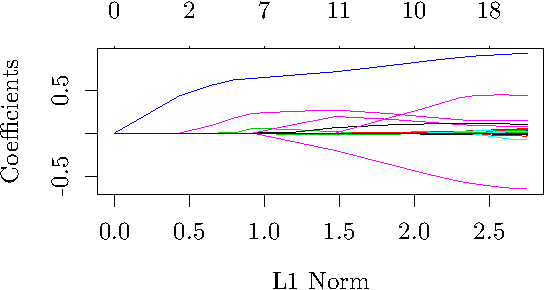
\includegraphics{tufte_files/figure-latex/lasso_sparse_matrix-1.pdf}
\caption{Lasso regression on the model.}
\end{marginfigure}

\subsection{Cross-validation to select best
model}\label{cross-validation-to-select-best-model}

After cross-validation only 11 variuables have non-zero coefficients and
are thus used during prediction. All other variabkes were shrunken to
zero.

\begin{Shaded}
\begin{Highlighting}[]
\NormalTok{cv.lasso <-}\StringTok{ }\KeywordTok{cv.glmnet}\NormalTok{(x, y, }\DataTypeTok{alpha =} \DecValTok{1}\NormalTok{, }\DataTypeTok{nfolds =} \DecValTok{5}\NormalTok{)}
\end{Highlighting}
\end{Shaded}

\begin{marginfigure}
 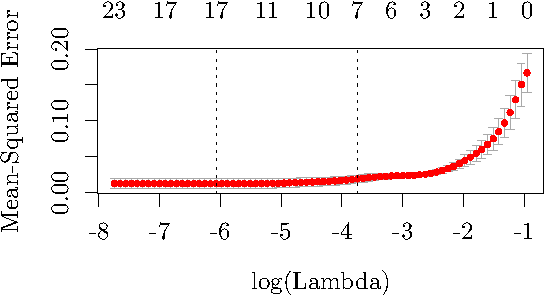
\includegraphics{tufte_files/figure-latex/lasso2-1.pdf}
\caption{Cross validation results for lasso regression. The best model only needs around 10 variables to describe the data with low error.}
\end{marginfigure}\begin{marginfigure}
 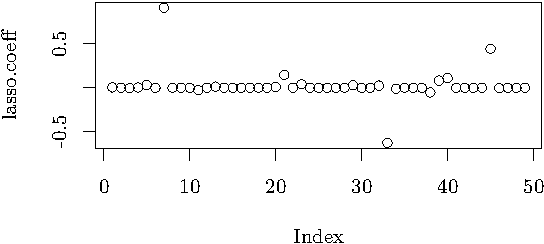
\includegraphics{tufte_files/figure-latex/lasso2-2.pdf}
\caption{The variables that have non-zero coefficients.}
\end{marginfigure}

\section{Answer}\label{answer}

\begin{itemize}
\itemsep1pt\parskip0pt\parsep0pt
\item
  the conversion is not by chance (significance between blank and enzyme
  treated groups)
\item
  The biggest influence on conversion has the presence of a catechgolic
  moiety (surprise, surprise !)
\item
  There is an effect of Mg and pH (main and interaction effect). However
  the statistical test don't support this notion. \(\rightarrow\)
  incubation time too large, this makes results badly interpretable !!!
  \(\rightarrow\) when catecholic moieties are excluded there is
  significance for Mg addition and possibly for pH; however no
  interaction
\item
  data is also very complex with possibly up to four factor interactions
\item
  regression tree used for interpretation \(\rightarrow\) pH and Mg can
  explain some of the variance
\end{itemize}

\begin{table}[ht]
\centering
\begin{tabular}{rlr}
  \toprule
 & variable & coefficient \\ 
  \midrule
1 & (Intercept) & 0.0128 \\ 
  2 & pHlow & -0.0144 \\ 
  3 & MgTRUE & 0.0017 \\ 
  4 & variantWT & 0.0258 \\ 
  5 & motifB & 0.8890 \\ 
  6 & pHlow:variantWT & -0.0096 \\ 
  7 & MgTRUE:variantWT & 0.0003 \\ 
  8 & MgTRUE:motifD & 0.0023 \\ 
  9 & variantWT:motifB & 0.1481 \\ 
  10 & variantWT:motifC & 0.0234 \\ 
  11 & pHlow:variantWT:motifB & 0.0237 \\ 
  12 & pHlow:variantY51RN202W:motifB & -0.5812 \\ 
  13 & pHlow:variantWT:motifC & -0.0005 \\ 
  14 & MgTRUE:variantWT:motifB & -0.0052 \\ 
  15 & MgTRUE:variantY51RN202W:motifB & 0.0944 \\ 
  16 & MgTRUE:variantWT:motifC & 0.1173 \\ 
  17 & MgTRUE:variantWT:motifD & 0.0031 \\ 
  18 & pHlow:MgTRUE:variantY51RN202W:motifB & 0.4286 \\ 
   \bottomrule
\end{tabular}
\caption{Variables and coefficients that were retained. Non-zero coefficients not shown.} 
\end{table}

\newpage

\section{Conversion of substrates}\label{conversion-of-substrates}

The conversion of the substrate in \% is of interest.

\subsection{Calculation of SAH and SAM
concentration}\label{calculation-of-sah-and-sam-concentration}

The SAH and SAM concentration were estimated from the area-under-curve
(AUC) of the SAM and SAH peaks. The displayed formula also already
include the conversion. \(x_\mathrm{SAH}\) is a direct measure for the
conversion.

\begin{marginfigure}
$$A_\mathrm{SAM} + A_\mathrm{SAM} = 1 \approx 500 \mathrm{uM}$$
$$x_\mathrm{SAH} = \frac{A_\mathrm{SAH}}{A_\mathrm{SAM} + A_\mathrm{SAM}}$$
$$c_\mathrm{SAH} = x_\mathrm{SAH} \times 500 \mathrm{uM}$$
\caption{Calculation of specific activity.}
\end{marginfigure}

0.4 mM substrate and 0.5 mM biologically active SAM were added. That
means the substrate conversion can be estimated by
\(conversion = \frac{0.4\mathrm{mM}}{0.5\mathrm{mM} \times x_\mathrm{SAH}}\).

\begin{marginfigure}
 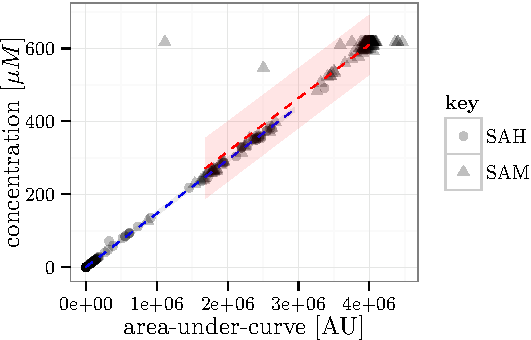
\includegraphics{tufte_files/figure-latex/concentration_estimation-1.pdf}
\caption{Estimated SAH and SAM concentration plotted against the AUC. Linear best-fit models with 95\% prediction intervals are included.}
\end{marginfigure}

\begin{table}[ht]
\centering
\begin{tabular}{rrrrr}
  \toprule
 & Estimate & Std. Error & t value & Pr($>$$|$t$|$) \\ 
  \midrule
(Intercept) & 5.9123E-01 & 2.8871E-01 & 2.0479E+00 & 4.2304E-02 \\ 
  area & 1.4674E-04 & 2.6532E-07 & 5.5305E+02 & 1.4152E-251 \\ 
   \bottomrule
\end{tabular}
\end{table}

\newpage
\#\# Calculation of the coefficients for
concentration\textasciitilde{}area bay bootstrapping

From the histogram of the coefficients obtained by the bootstrap it is
clear that there is a non-gaussian distribution for the coefficients for
SAM. This could be due to the fact that there is a huge amount of
samples with high SAM concentrations, which produces bias.

\begin{Shaded}
\begin{Highlighting}[]
\NormalTok{boot.fn <-}\StringTok{ }\NormalTok{function(data, index) \{}
    \NormalTok{data <-}\StringTok{ }\NormalTok{data[index, ]}
    \NormalTok{data %<>%}\StringTok{ }\KeywordTok{mutate}\NormalTok{(}\DataTypeTok{x =} \NormalTok{(area/flavon)/((SAH/flavon) +}\StringTok{ }
\StringTok{        }\NormalTok{(SAM/flavon)), }\DataTypeTok{concentration =} \NormalTok{(x *}\StringTok{ }\DecValTok{500}\NormalTok{/}\FloatTok{0.81}\NormalTok{))  }\CommentTok{# the total concentration of SAm is needed (R+L) --> 0.81 of SAm is biologicalle active}
    \KeywordTok{return}\NormalTok{(}\KeywordTok{coef}\NormalTok{(}\KeywordTok{lm}\NormalTok{(concentration ~}\StringTok{ }\NormalTok{area, }\DataTypeTok{data =} \NormalTok{data)))}
\NormalTok{\}}


\NormalTok{lm.boot.sah <-}\StringTok{ }\KeywordTok{boot}\NormalTok{(WEB346.CV %>%}\StringTok{ }\KeywordTok{select}\NormalTok{(SAH, }
    \NormalTok{SAM, flavon) %>%}\StringTok{ }\KeywordTok{mutate}\NormalTok{(}\DataTypeTok{area =} \NormalTok{SAH), boot.fn, }
    \DecValTok{1000}\NormalTok{)}
\NormalTok{lm.boot.sam <-}\StringTok{ }\KeywordTok{boot}\NormalTok{(WEB346.CV %>%}\StringTok{ }\KeywordTok{select}\NormalTok{(SAH, }
    \NormalTok{SAM, flavon) %>%}\StringTok{ }\KeywordTok{mutate}\NormalTok{(}\DataTypeTok{area =} \NormalTok{SAM), boot.fn, }
    \DecValTok{1000}\NormalTok{)}

\NormalTok{pred.SAH <-}\StringTok{ }\KeywordTok{data.frame}\NormalTok{(}\DataTypeTok{area =} \NormalTok{WEB346.CV$SAH, }\DataTypeTok{concentration =} \NormalTok{WEB346.CV$SAH *}\StringTok{ }
\StringTok{    }\NormalTok{lm.boot.sah$t0[}\DecValTok{2}\NormalTok{] +}\StringTok{ }\NormalTok{lm.boot.sah$t0[}\DecValTok{1}\NormalTok{])}
\NormalTok{pred.SAM <-}\StringTok{ }\KeywordTok{data.frame}\NormalTok{(}\DataTypeTok{area =} \NormalTok{WEB346.CV$SAM, }\DataTypeTok{concentration =} \NormalTok{WEB346.CV$SAM *}\StringTok{ }
\StringTok{    }\NormalTok{lm.boot.sam$t0[}\DecValTok{2}\NormalTok{] +}\StringTok{ }\NormalTok{lm.boot.sam$t0[}\DecValTok{1}\NormalTok{])}
\end{Highlighting}
\end{Shaded}

\begin{figure}
 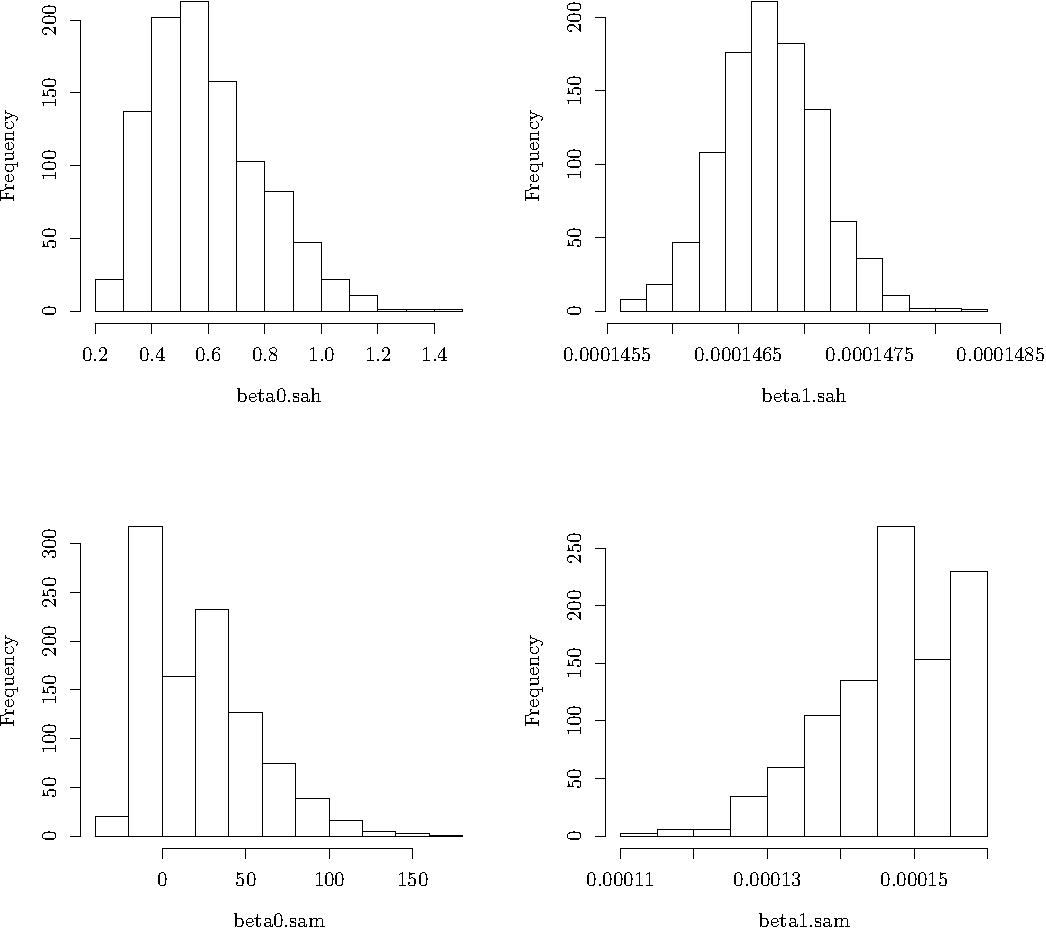
\includegraphics{tufte_files/figure-latex/unnamed-chunk-11-1.pdf}
\caption{Histogram of coefficient values obtained by bootstrap with n=1000}
\end{figure}\begin{figure}
 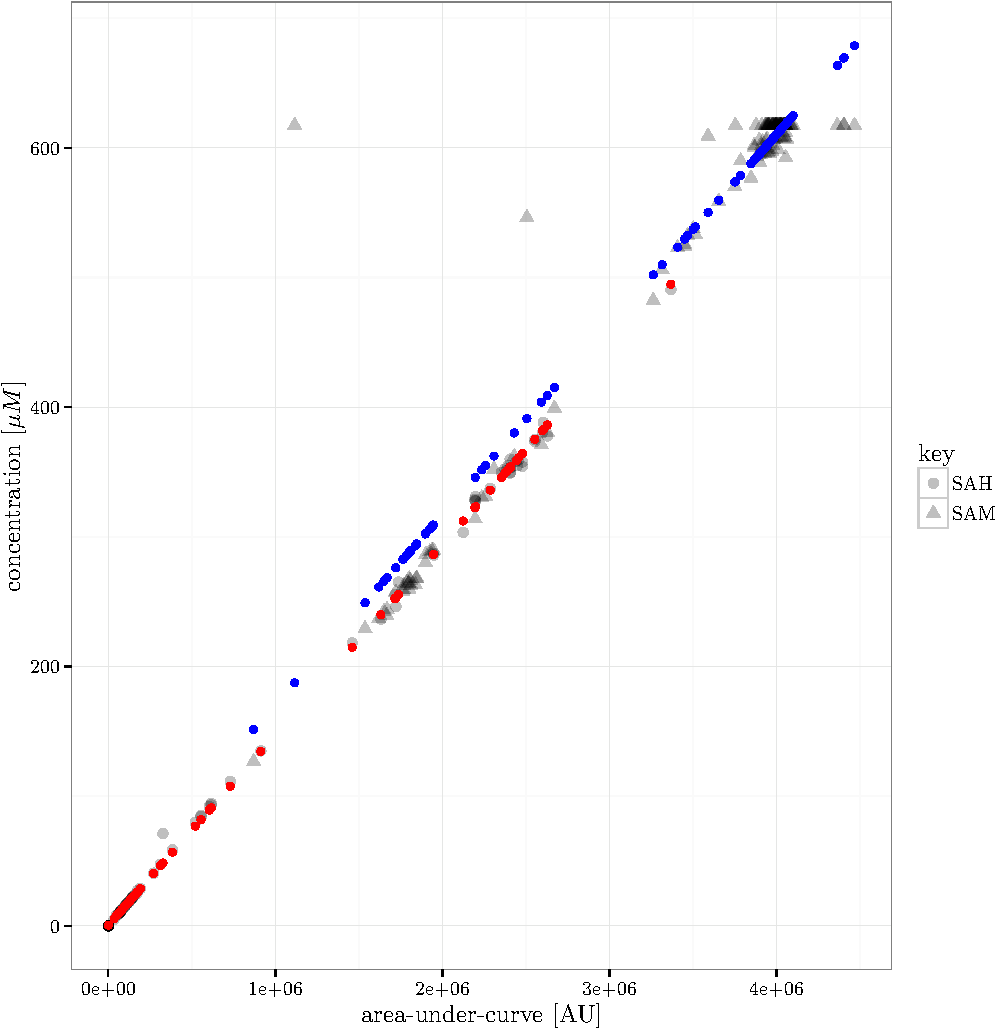
\includegraphics{tufte_files/figure-latex/unnamed-chunk-11-2.pdf}
\caption{Calculated data from the bootstrap.}
\end{figure}

\begin{verbatim}
## 
## ORDINARY NONPARAMETRIC BOOTSTRAP
## 
## 
## Call:
## boot(data = WEB346.CV %>% select(SAH, SAM, flavon) %>% mutate(area = SAH), 
##     statistic = boot.fn, R = 1000)
## 
## 
## Bootstrap Statistics :
##         original       bias     std. error
## t1* 0.5912346000 4.456157e-03 1.974150e-01
## t2* 0.0001467374 5.576398e-09 3.876305e-07
\end{verbatim}

\begin{verbatim}
## 
## ORDINARY NONPARAMETRIC BOOTSTRAP
## 
## 
## Call:
## boot(data = WEB346.CV %>% select(SAH, SAM, flavon) %>% mutate(area = SAM), 
##     statistic = boot.fn, R = 1000)
## 
## 
## Bootstrap Statistics :
##         original        bias     std. error
## t1* 2.405931e+01 -1.042784e+00 3.324905e+01
## t2* 1.465407e-04  2.895498e-07 8.687305e-06
\end{verbatim}

\newpage

\section{Phenolic substrates}\label{phenolic-substrates}

\begin{marginfigure}
 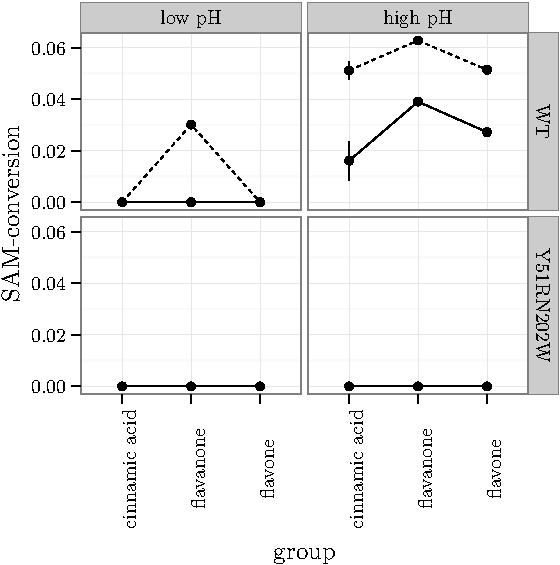
\includegraphics{tufte_files/figure-latex/plot_conversion_phenol-1.pdf}
\caption{Comparison of conversion of phenolic substrates. dashed line -- 10 mM Mg, solid line -- no Mg}
\end{marginfigure}

\section{3'-O-methyl substrates}\label{o-methyl-substrates}

\begin{marginfigure}
 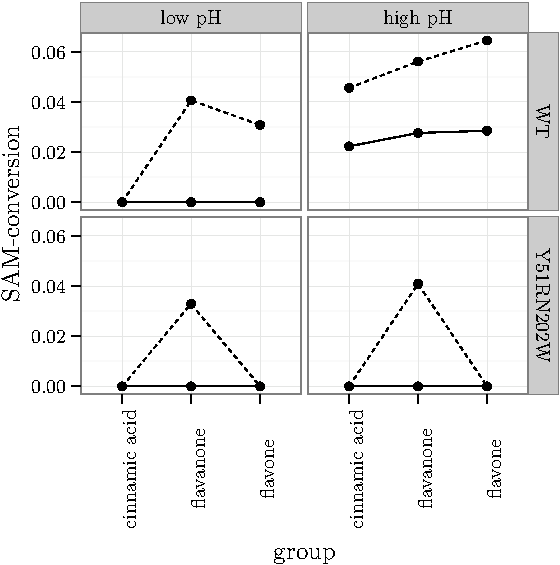
\includegraphics{tufte_files/figure-latex/plot_conversion_3Ome-1.pdf}
\caption{Comparison of conversion of 3'-O-methyl substrates. dashed line -- 10 mM Mg, solid line -- no Mg}
\end{marginfigure}

\section{4'-O-methyl substrates}\label{o-methyl-substrates-1}

\begin{marginfigure}
 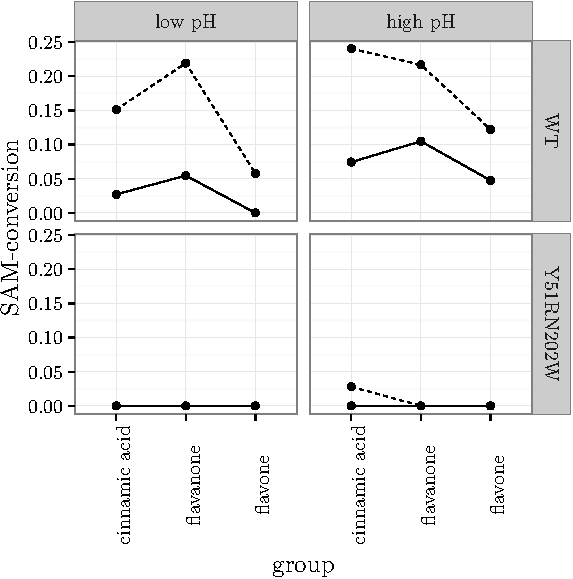
\includegraphics{tufte_files/figure-latex/plot_conversion_4Ome-1.pdf}
\caption{Comparison of conversion of 4'-O-methyl substrates. dashed line -- 10 mM Mg, solid line -- no Mg}
\end{marginfigure}

\newpage

\section{catecholic substrates}\label{catecholic-substrates}

\begin{marginfigure}
 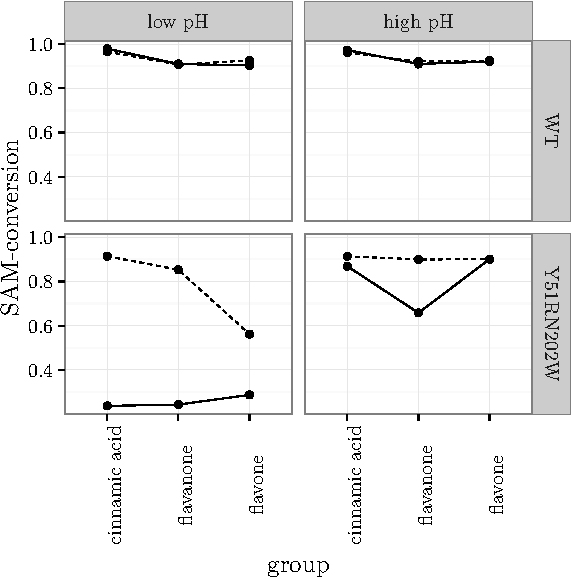
\includegraphics{tufte_files/figure-latex/plot_conversion_catechol-1.pdf}
\caption{Comparison of conversion of catecholic substrates. dashed line -- 10 mM Mg, solid line -- no Mg}
\end{marginfigure}

\section{Calculation of all
conversions}\label{calculation-of-all-conversions}

\begin{table}[ht]
\centering
\begin{tabular}{rllrll}
  \toprule
 & substrate & variant & max & at.pH & at.Mg \\ 
  \midrule
1 & 1 & WT & 0.06 & high & TRUE \\ 
  2 & 2 & WT & 0.94 & high & TRUE \\ 
  3 & 3 & WT & 0.22 & low & TRUE \\ 
  4 & 4 & WT & 0.06 & high & TRUE \\ 
  5 & 5 & WT & 0.05 & high & TRUE \\ 
  6 & 6 & WT & 0.95 & low & TRUE \\ 
  7 & 7 & WT & 0.12 & high & TRUE \\ 
  8 & 8 & WT & 0.07 & high & TRUE \\ 
  9 & 9 & WT & 0.06 & high & TRUE \\ 
  10 & 10 & WT & 0.06 & high & TRUE \\ 
  11 & 11 & WT & 0.04 & high & TRUE \\ 
  12 & 12 & WT & 1.00 & low & FALSE \\ 
  13 & 14 & WT & 0.25 & high & TRUE \\ 
  14 & 13 & WT & 0.05 & high & TRUE \\ 
  15 & 15 & WT & 0.06 & high & TRUE \\ 
  16 & 16 & WT & 0.93 & high & FALSE \\ 
  17 & 17 & WT & 1.29 & low & FALSE \\ 
   \bottomrule
\end{tabular}
\end{table}\begin{table}[ht]
\centering
\begin{tabular}{rllrll}
  \toprule
 & substrate & variant & max & at.pH & at.Mg \\ 
  \midrule
1 & 1 & Y51RN202W &  &  &  \\ 
  2 & 2 & Y51RN202W & 0.92 & high & TRUE \\ 
  3 & 3 & Y51RN202W &  &  &  \\ 
  4 & 4 & Y51RN202W & 0.04 & high & TRUE \\ 
  5 & 5 & Y51RN202W &  &  &  \\ 
  6 & 6 & Y51RN202W & 0.92 & high & FALSE \\ 
  7 & 7 & Y51RN202W &  &  &  \\ 
  8 & 8 & Y51RN202W &  &  &  \\ 
  9 & 9 & Y51RN202W &  &  &  \\ 
  10 & 10 & Y51RN202W &  &  &  \\ 
  11 & 11 & Y51RN202W &  &  &  \\ 
  12 & 12 & Y51RN202W & 0.93 & low & TRUE \\ 
  13 & 14 & Y51RN202W & 0.03 & high & TRUE \\ 
  14 & 13 & Y51RN202W &  &  &  \\ 
  15 & 15 & Y51RN202W & 0.07 & high & TRUE \\ 
  16 & 16 & Y51RN202W & 0.86 & high & TRUE \\ 
  17 & 17 & Y51RN202W & 1.02 & low & TRUE \\ 
   \bottomrule
\end{tabular}
\end{table}

\begin{figure}
 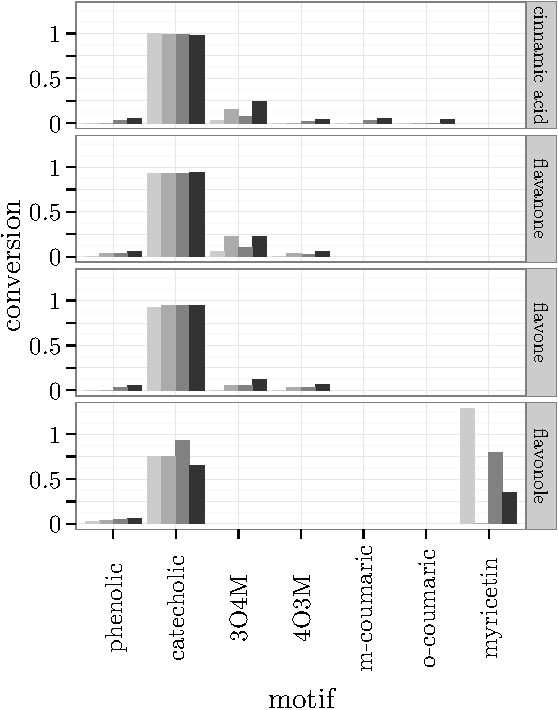
\includegraphics{tufte_files/figure-latex/unnamed-chunk-14-1.pdf}
\caption{Wild-type conversions. colors from light to dark: low/no, low/yes, high/no, high/yes}
\end{figure}\begin{figure}
 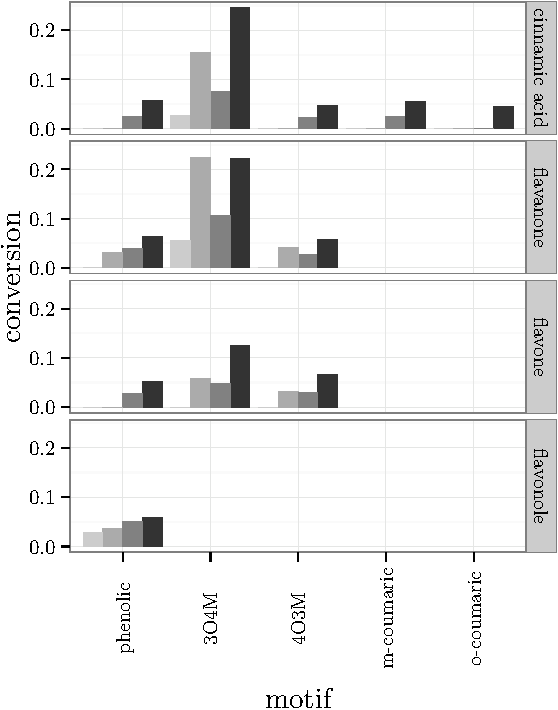
\includegraphics{tufte_files/figure-latex/unnamed-chunk-14-2.pdf}
\caption{Same as above, but some data is omitted.}
\end{figure}\begin{figure}
 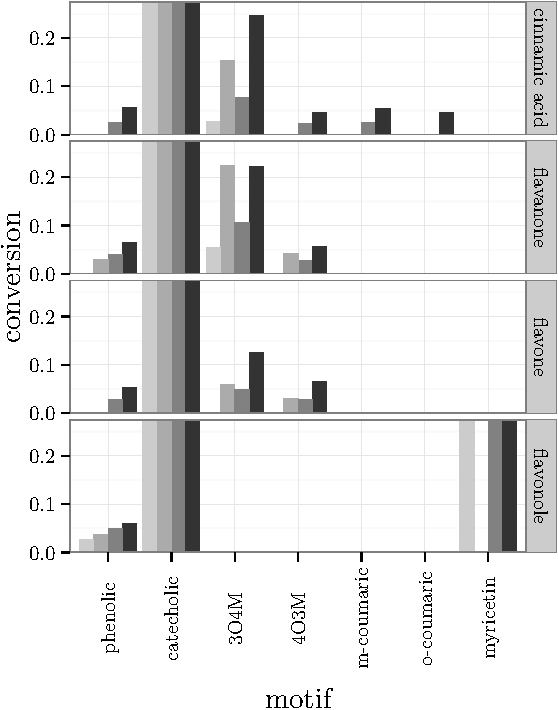
\includegraphics{tufte_files/figure-latex/unnamed-chunk-14-3.pdf}
\caption{4'-selective variant conversions. colors from light to dark: low/no, low/yes, high/no, high/yes}
\end{figure}\begin{figure}
 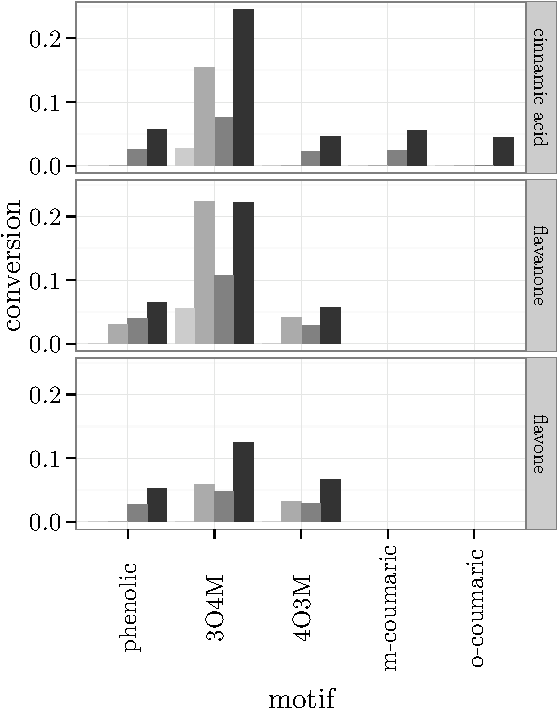
\includegraphics{tufte_files/figure-latex/unnamed-chunk-14-4.pdf}
\caption{Wild-type conversions. colors from light to dark: low/no, low/yes, high/no, high/yes}
\end{figure}


\end{document}
